\documentclass[mathserif,serif]{beamer}
\usepackage[ngerman]{babel}
%\usepackage[scale=0.75]{geometry}
\usepackage{graphics}
\usepackage{graphicx}
\usepackage{amsmath}
\usepackage{amssymb}
\usepackage{subfigure} 
\usepackage[utf8]{inputenc}
\usepackage{amsmath}
\usepackage{amsfonts}
\usepackage{amssymb}
\usepackage{fancyhdr}
\usepackage[hang, center, nooneline]{caption}
\usepackage{epstopdf}
\usepackage{color}
\usepackage{subfigure}
\usepackage{wrapfig}
\usepackage{color}															 
\usepackage{colortbl}
\usepackage{siunitx}
\usepackage{fancybox}
\usepackage{relsize}
\usepackage{booktabs}
\usepackage{tikz}
\usepackage{textpos}
\usepackage{colortbl}

\definecolor{TUeRed}{RGB}{170,0,0}
\definecolor{TUeBlue}{RGB}{0,68,170}

\addtobeamertemplate{frametitle}{}{% 
\begin{textblock*}{100mm}(.95\textwidth,-1cm) \tikz {\fill[white] (0,0) -- %
(2cm,0) -- (2cm,1.1cm) -- (0.5cm,1.1cm) -- cycle;\node[TUeBlue] at %
(0.8cm,0.5cm) {\normalsize\insertframenumber};} \end{textblock*} }

\setbeamercolor{frametitle}{bg=TUeBlue}
\setbeamercolor{frametitle}{fg=white}

  
%EIGENE FOOTLINE (OHNE GESAMTSEITENZAHL) 
%\setbeamertemplate{footline} 
%{ 
%\leavevmode% 
%\hbox{% 
%\begin{beamercolorbox}[wd=.333333\paperwidth,ht=2.25ex,dp=1ex,center]{author in head/foot}% 
%\usebeamerfont{author in head/foot}\insertshortauthor~~ 
%\end{beamercolorbox}% 
%\begin{beamercolorbox}[wd=.333333\paperwidth,ht=2.25ex,dp=1ex,center]{title in head/foot}% 
%\usebeamerfont{title in head/foot}\insertshorttitle 
%\end{beamercolorbox}% 
%\begin{beamercolorbox}[wd=.333333\paperwidth,ht=2.25ex,dp=1ex,right]{date in head/foot}% 
%\usebeamerfont{date in head/foot}\insertshortdate{}
%\end{beamercolorbox}}% 
%\vskip0pt% 
%}

\setbeamertemplate{footline}[text line]{%
  \parbox{\linewidth}{\vspace*{-8pt}\hspace*{-5mm}\insertshortauthor\hfill Particles in a Potential\hfill\insertdate}}

\beamertemplatenavigationsymbolsempty

\author{Christopher Deutsch and Philip Hauer}
\title{Particles in a Potential}
\date{30. March 2016}
\subtitle{{\small Computational Physics}}

\begin{document}
\frame[plain]{\titlepage}
\setcounter{framenumber}{0}
\begin{frame}
	\frametitle{Introduction - Particles in a Potential}
	
		
			Core of this project:
			\begin{itemize}
			\setlength\itemsep{1.5em}
				\item particles in a box
				\item interaction via potential
				\item analysis with a Random-Walk Metropolis algorithm
				\item study of temperature dependence
			\end{itemize}
			
\end{frame}


% % % % % % % % % % % % Philip Intro

%Hier Folien


% % % % % % % % % % % % Chris Background & Implementation

%Hier Folien
\begin{frame}{Canonical ensemble}
	\begin{columns}
		\column[c]{0.5\textwidth}
			\begin{itemize}
				\setlength\itemsep{1.5em}
				\item statistical ensemble
				\item systems with constant:
				\begin{itemize}
					\item number of particles~$N$
					\item volume~$V$
					\item temperature~$T$
				\end{itemize}
				
				\item probabilistic description
			\end{itemize}
		
			
		\column[c]{0.5\textwidth}
			\centering
			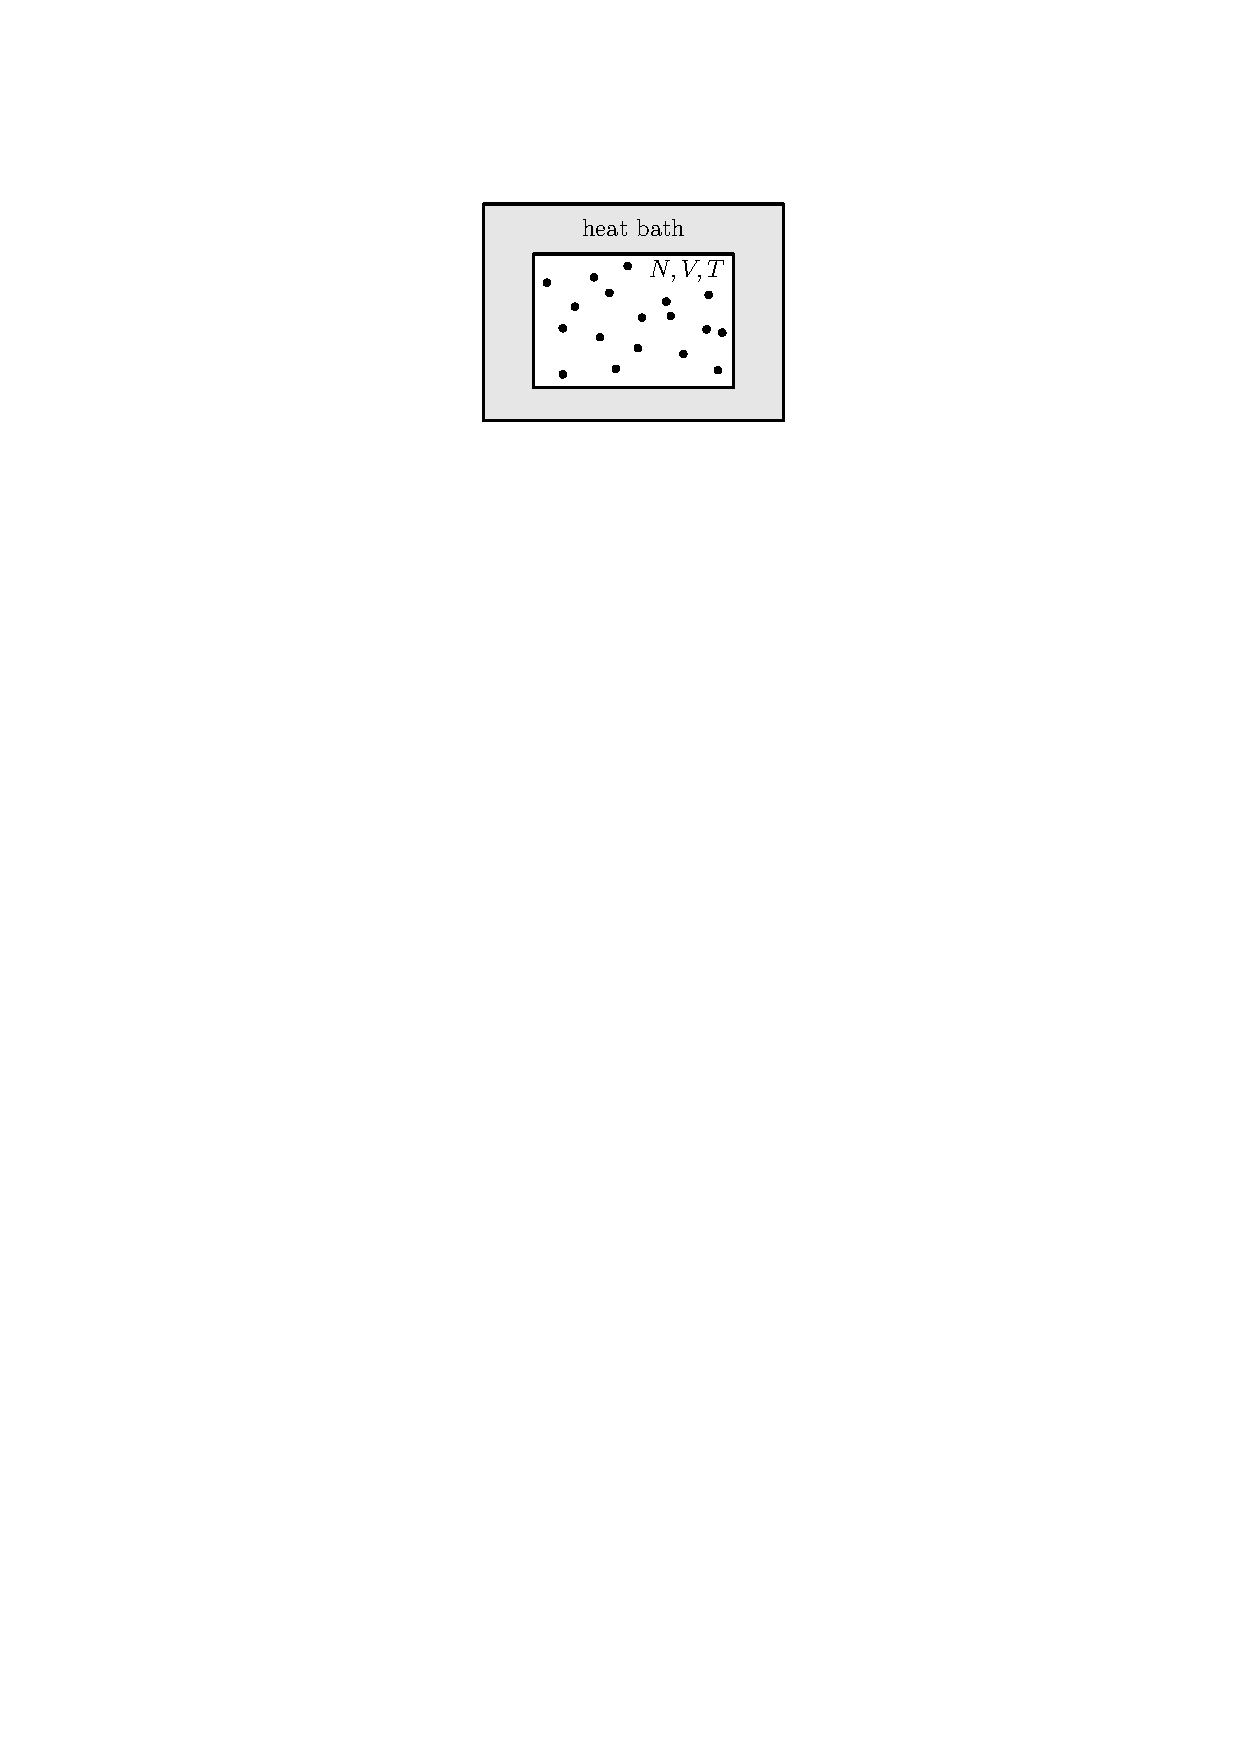
\includegraphics[width=0.9\textwidth]{./figures/canonical_ensemble.pdf}
		
	\end{columns}
\end{frame}

\begin{frame}{Canonical ensemble}
	\begin{itemize}
		\setlength\itemsep{2.0em}
		\item probability density:
		\begin{align*}
			P(E) = \frac{1}{Z} \exp\left[ - \beta E \right] \qquad \beta := \frac{1}{k_\mathrm{B} T}
		\end{align*}
		$E$: total energy of system\\
		$Z$: canonical partition function
		
		\item examine temperature dependence:
		\begin{itemize}
			\item sample states from distribution
			\item calculate expectation values of observables
		\end{itemize}
	\end{itemize}
\end{frame}

\begin{frame}{Metropolis algorithm}
	\begin{itemize}
		\setlength\itemsep{1.5em}
		\item MCMC method for sampling from (complicated) distributions
		\item correlated sequence of random samples
		\begin{itemize}
			\item used to approximate distribution
		\end{itemize}
		\item Random-Walk Metropolis
	\end{itemize}

\end{frame}

\begin{frame}{Random-Walk Metropolis algorithm}
	Given target density $P(x)$ and initial state $x_0$:
	\vspace*{0.2cm}
	\begin{enumerate}
		\setlength{\itemsep}{1.5em}
		\item Trial change:
		\begin{itemize}
			\item generate new state $y$ according to symmetric proposal distribution $q(Y|x_n)$
		\end{itemize}
		
		\item Accept-reject:
		\begin{itemize}
			\item accept with probability:
			\begin{align*}
				\alpha = \min\left\{ \frac{P(y)}{P(x_n)}, 1 \right\}
			\end{align*}
		\end{itemize}
		
		\item Repeat
	\end{enumerate}		
\end{frame}

\begin{frame}{Implementation}
	\begin{columns}
		\column[c]{0.5\textwidth}
			\begin{itemize}
				\setlength{\itemsep}{1.5em}
				\item<2-> random initial state
				\item<3-> select particle at random and calculate~$E_\mathrm{cur.}$
				\item<4-> propose new state in box
				\begin{itemize}
					\item<5-> calculate~$E_\mathrm{prop.}$
				\end{itemize}
				\item<6-> accept with probability:
				\begin{align*}
					\alpha &= \frac{P(E_\mathrm{prop.})}{P(E_\mathrm{cur.})}\\[.5em]
					       &= \exp\left[ -\beta (E_\mathrm{prop.} - E_\mathrm{cur.}) \right]
				\end{align*}
			\end{itemize}
		\column[c]{0.5\textwidth}
			\centering
			\includegraphics<1>{./figures/impl_01.pdf}
			\includegraphics<2>{./figures/impl_02.pdf}
			\includegraphics<3>{./figures/impl_03.pdf}
			\includegraphics<4>{./figures/impl_04.pdf}
			\includegraphics<5>{./figures/impl_05.pdf}
			\includegraphics<6>{./figures/impl_06.pdf}
	\end{columns}
\end{frame}


% % % % % % % % % % % % Philip Intro Tempdep & Potentials

\begin{frame}
	\frametitle{Temperature Dependence -- Settings}
	\begin{columns}
		\column[c]{0.5\textwidth}
		Parameters:
		\begin{itemize}
			\setlength{\itemsep}{0.7em}
			\item<2-> dimensions
			\item<3-> size of box
			\item<4-> number of particles
			\item<5-> thermodynamical $\beta$
			\item<6-> $\Delta$ (for proposal distribution)
			\item<7-> inter-particle potential
		\end{itemize}
		\column[c]{0.5\textwidth}
			\centering
			\includegraphics<1>{./figures/Empty_setting.pdf}
			\includegraphics<2>{./figures/Dim_setting_all.pdf}
			\includegraphics<3>{./figures/Size_setting_all.pdf}
			\includegraphics<4>{./figures/N_setting_all.pdf}
			\includegraphics<5>{./figures/Beta_setting_all.pdf}
			\includegraphics<6>{./figures/Delta_setting_all.pdf}
			\includegraphics<7>{./figures/Empty_setting.pdf}
	\end{columns}
\end{frame}

\begin{frame}{Potentials -- Coulomb with hard core}
	\centering
	$V_{ij} = \frac{q_i q_j}{| \mathbf{r}_i - \mathbf{r}_j |} + \frac{1}{| \mathbf{r}_i - \mathbf{r}_j |^8}$
	
	
	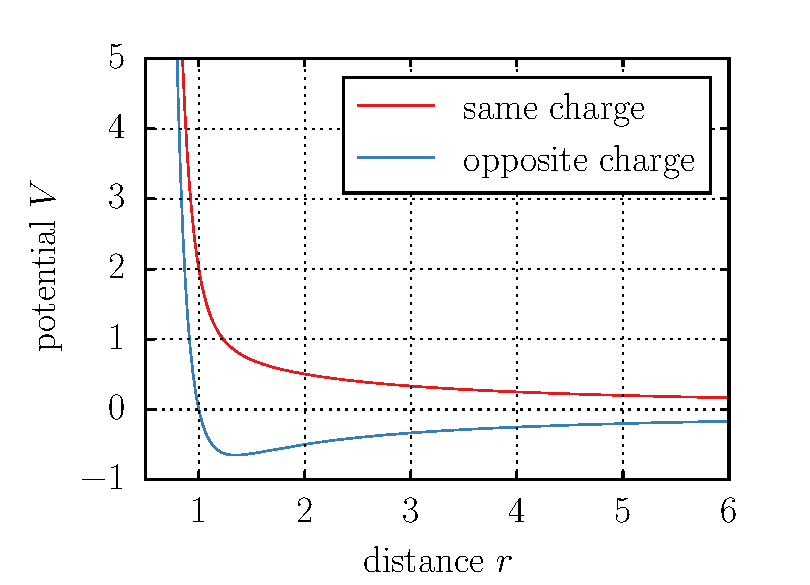
\includegraphics[height=0.5\textheight]{./figures/potential_coulomb.pdf}
	\begin{columns}
		\column[c]{0.5\textwidth}
			\begin{itemize}
				\item hard core for $r < 1$
				\item coulomb dominates for $r \gg 1$
			\end{itemize}
		\column[c]{0.5\textwidth}
			\begin{itemize}
				\item attractive for opposite charges ($r > 1$)
				\item minimum at $r\approx 1.35$
			\end{itemize}
	\end{columns}
	
\end{frame}

\begin{frame}{Potentials -- Lennard-Jones}
	\centering
	$V_{ij} = \frac{1}{| \mathbf{r}_i - \mathbf{r}_j |^{12}} - \frac{1}{| \mathbf{r}_i - \mathbf{r}_j |^6}$
	
	
	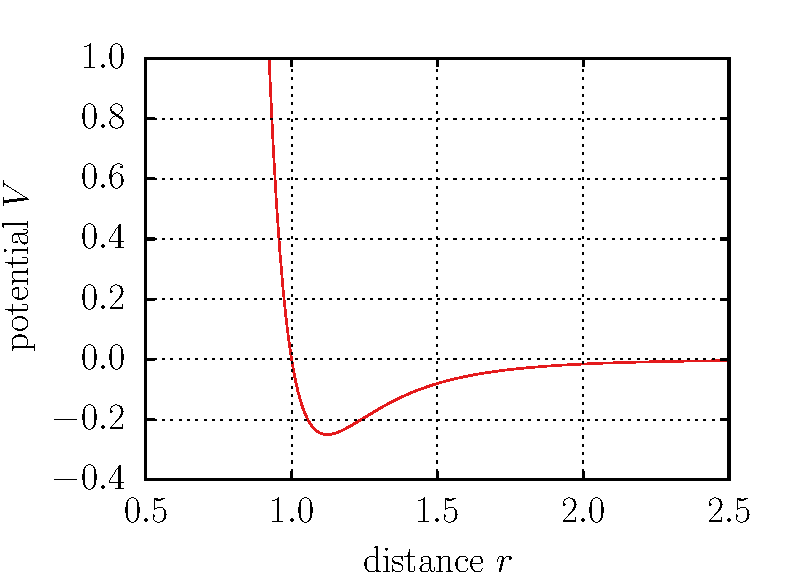
\includegraphics[height=0.5\textheight]{./figures/potential_lennard_jones.pdf}
	\begin{columns}
		\column[c]{0.5\textwidth}
			\begin{itemize}
				\item neutral particles
				\item extremely short ranged
			\end{itemize}
		\column[c]{0.5\textwidth}
			\begin{itemize}
				\item always attractive ($r > 1$)
				\item minimum at $r\approx 1.12$
			\end{itemize}
	\end{columns}
	
\end{frame}

% % % % % % % % % % % % Chris 4.2 Analysis & avg pair distance

%Hier Folien
\begin{frame}{Analysis of the temperature dependence}
	\begin{itemize}
		\setlength{\itemsep}{1.5em}
		\item observable indicative of phase
		\begin{itemize}
			\item average pair-distance
			\begin{align*}
			d = \frac{1}{N(N-1)}\sum_{i \neq j} |\mathbf{r}_i - \mathbf{r}_i|
			\end{align*}
			\item evaluated every 20th sample
		\end{itemize}
		\item multiple sequences of random samples
		\begin{itemize}
			\item mean of expectation values
			\item standard deviation
			\item 0.05/0.95-quantiles
		\end{itemize}
	\end{itemize}
	
\end{frame}


% % % % % % % % % % % % Philip Coulomb 2D 3D & Visualizations
\begin{frame}
	\frametitle{Results -- Coulomb 2D}
	\centering	
	\begin{figure}
	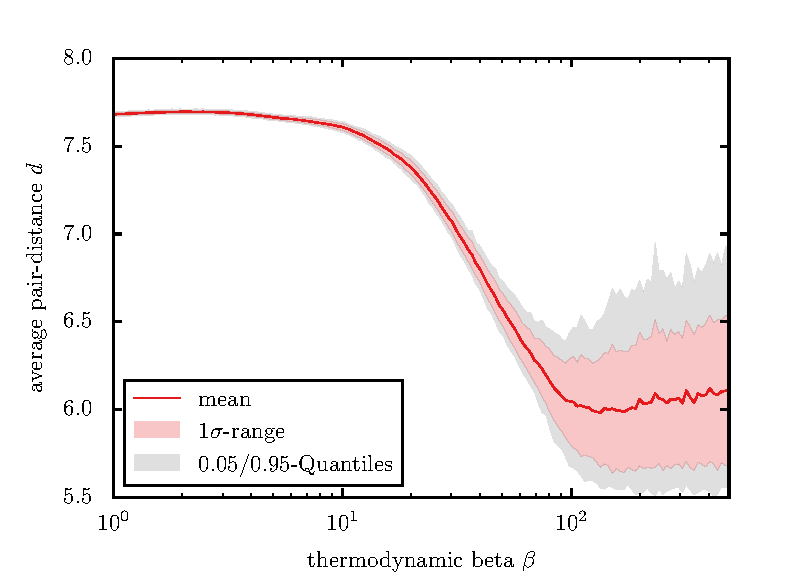
\includegraphics[width=\textwidth]{../report/figures/temp_dep_coulomb2d.pdf}
	\pause
	\put(-254,140){$\beta = 2$}
	\put(-239,152){\vector(0,1){17}}
	\end{figure}
\end{frame}

\begin{frame}
	\frametitle{Results -- Coulomb 2D @ $\beta=2$}
	\centering
	\begin{columns}	
	\column[c]{0.6\textwidth}
	\begin{figure}
	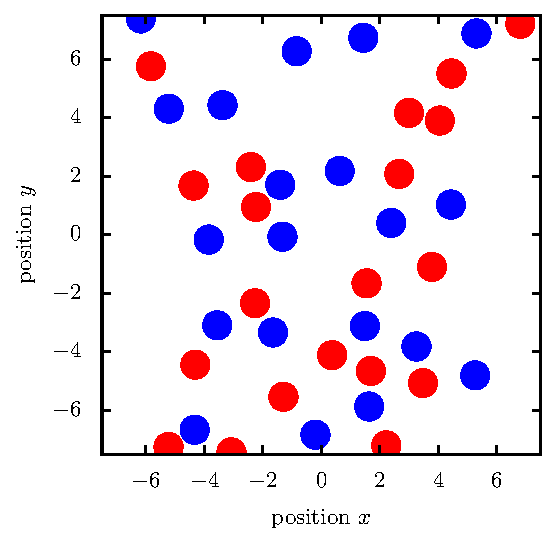
\includegraphics[width=\textwidth]{../report/figures/Plasma_1_beta_2.pdf}
	\end{figure}
	\column[c]{0.45\textwidth}
	\begin{itemize}
	\setlength{\itemsep}{1.3em}
	\item plasma-like state
	\item no regular structure
	\item distributed over whole box
	\item large avg. pair-distance
	\end{itemize}
\end{columns}
\end{frame}


\begin{frame}
	\frametitle{Results -- Coulomb 2D}
	\centering	
	\begin{figure}
	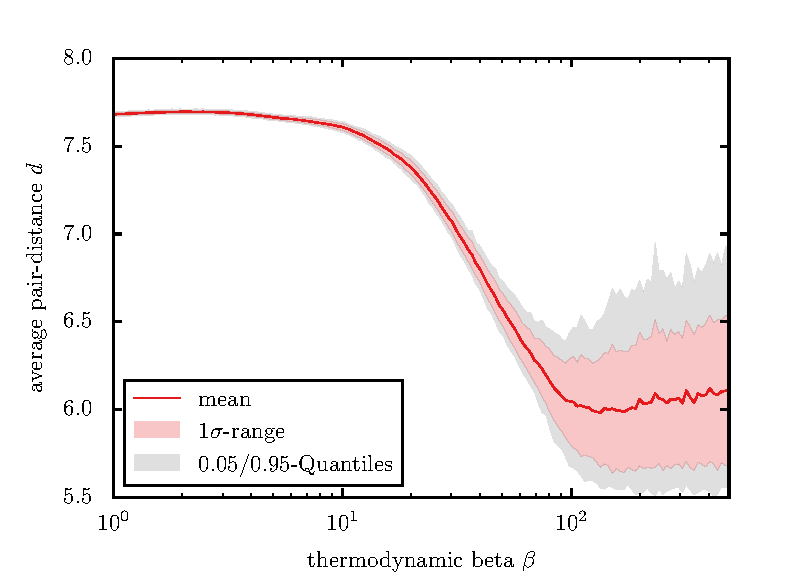
\includegraphics[width=\textwidth]{../report/figures/temp_dep_coulomb2d.pdf}
	\put(-192.5,138){$\beta = 10$}
	\put(-177.5,150){\vector(0,1){17}}
	\end{figure}
\end{frame}

\begin{frame}
	\frametitle{Results -- Coulomb 2D @ $\beta=10$}
	\centering
	\begin{columns}	
	\column[c]{0.6\textwidth}
	\begin{figure}
	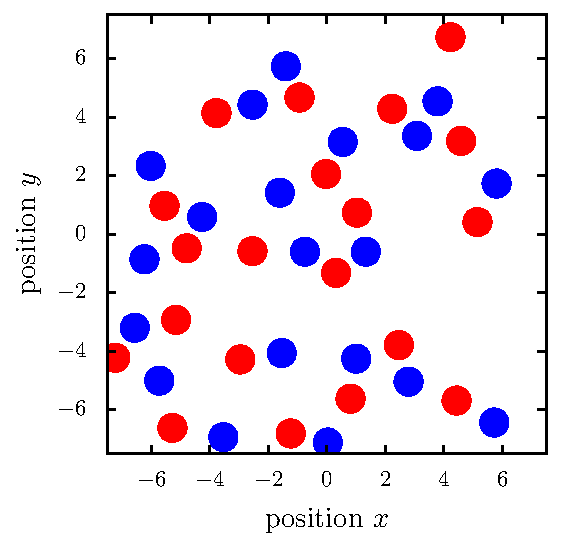
\includegraphics[width=\textwidth]{../report/figures/Gas_1_beta_10.pdf}
	\end{figure}
	\column[c]{0.5\textwidth}
	\begin{itemize}
	\setlength{\itemsep}{1.3em}
	\item gaseous state (molecular gas)
	\item negative and positive charged particles form pairs
	\item distributed over whole box
	\item again: large avg. pair-distance
	\end{itemize}
\end{columns}
\end{frame}

\begin{frame}
	\frametitle{Results -- Coulomb 2D}
	\centering	
	\begin{figure}
	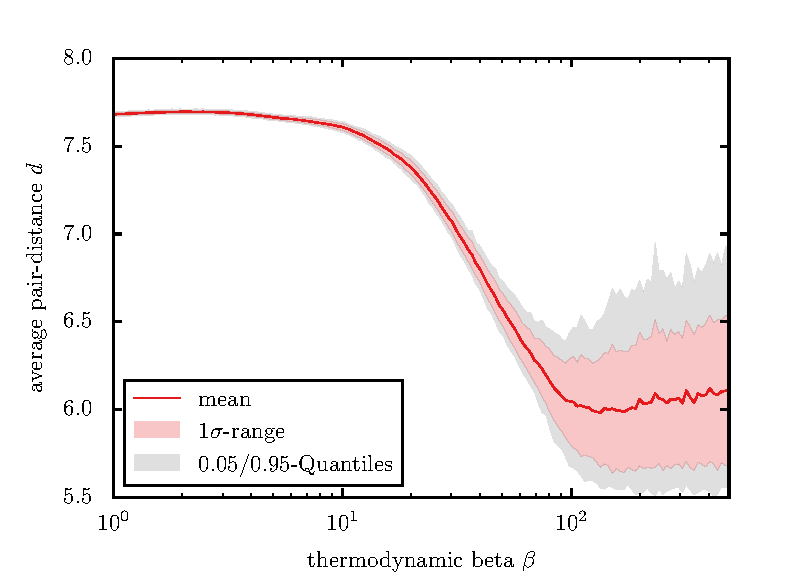
\includegraphics[width=\textwidth]{../report/figures/temp_dep_coulomb2d.pdf}
	\put(-134,150){$\beta = 40$}
	\put(-119,147){\vector(0,-1){17}}
	\end{figure}
\end{frame}

\begin{frame}
	\frametitle{Results -- Coulomb 2D @ $\beta=40$}
	\centering
	\begin{columns}	
	\column[c]{0.6\textwidth}
	\begin{figure}
	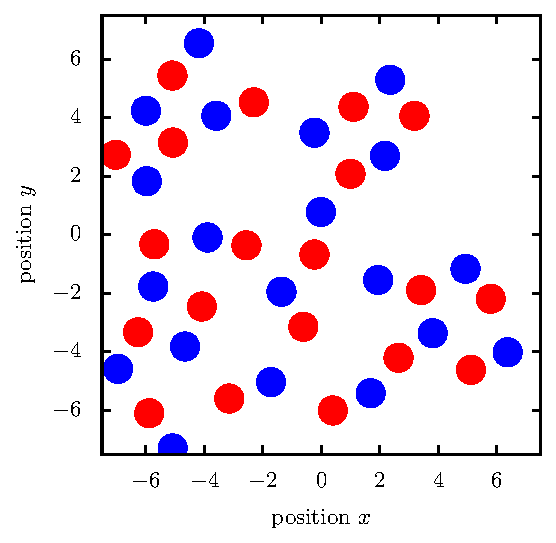
\includegraphics[width=\textwidth]{../report/figures/Fluid_1_beta_40.pdf}
	\end{figure}
	\column[c]{0.5\textwidth}
	\begin{itemize}
	\setlength{\itemsep}{1.3em}
	\item fluid state	
	\item no regular structure
	\item few chains formed
	\item smaller avg. pair-distance
	\end{itemize}
\end{columns}
\end{frame}

\begin{frame}
	\frametitle{Results -- Coulomb 2D}
	\centering	
	\begin{figure}
	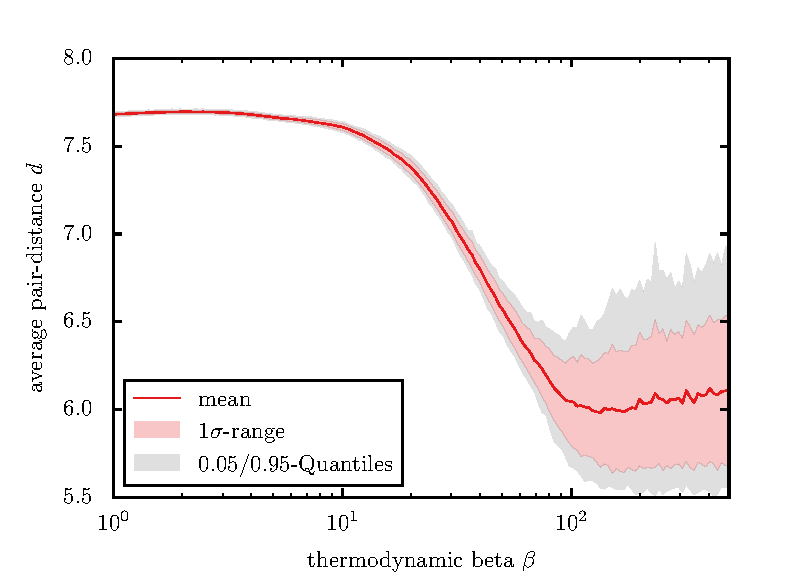
\includegraphics[width=\textwidth]{../report/figures/temp_dep_coulomb2d.pdf}
	\put(-80,97){$\beta = 500$}
	\put(-41,94){\vector(1,-2){10}}
	\end{figure}
\end{frame}

\begin{frame}
	\frametitle{Results -- Coulomb 2D @ $\beta=500$}
	\centering
	\begin{columns}	
	\column[c]{0.6\textwidth}
	\begin{figure}
	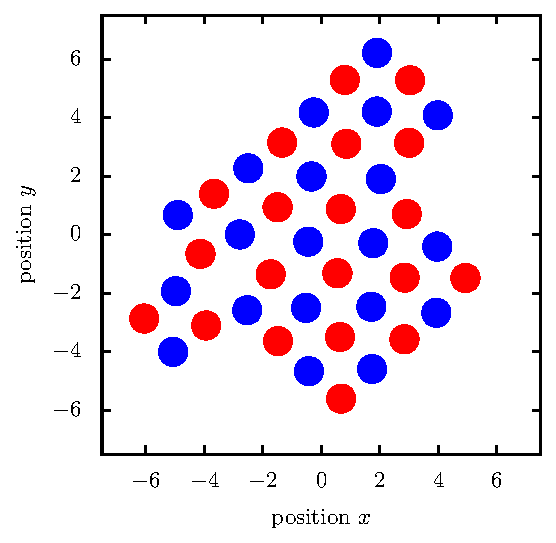
\includegraphics[width=\textwidth]{../report/figures/Kristall_3_beta_500.pdf}
	\end{figure}
	\column[c]{0.5\textwidth}
	\begin{itemize}
	\setlength{\itemsep}{1.5em}
	\item solid state
	\item regular lattice
	\item small avg. pair-distance	
	\end{itemize}
\end{columns}
\end{frame}


\begin{frame}
	\frametitle{Results -- Coulomb 2D @ $\beta=500$}
	\centering
	\begin{columns}	
	\column[c]{0.6\textwidth}
	\begin{figure}
	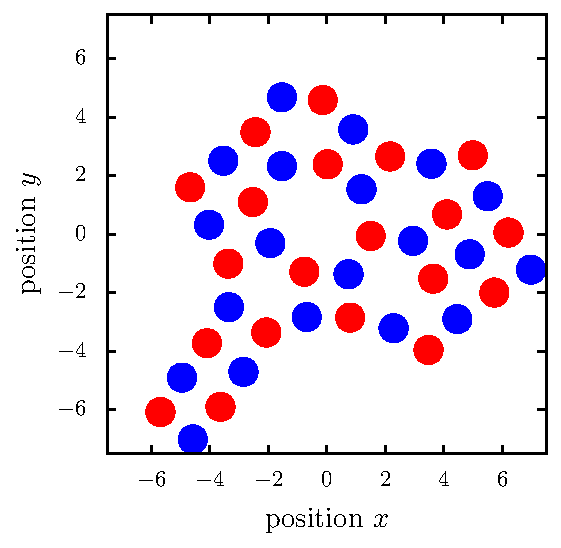
\includegraphics[width=\textwidth]{../report/figures/Kristall_4_beta_500.pdf}
	\end{figure}
	\column[c]{0.5\textwidth}
	\begin{itemize}
	\setlength{\itemsep}{1.5em}
	\item solid state
	\item (mostly) regular lattice
	\item avg. pair-distance is now larger
	\end{itemize}
	\vspace{2em}
	Defects are a source of the large uncertainty!
\end{columns}
\end{frame}

\begin{frame}
	\frametitle{Results -- Coulomb 2D}
	\centering
	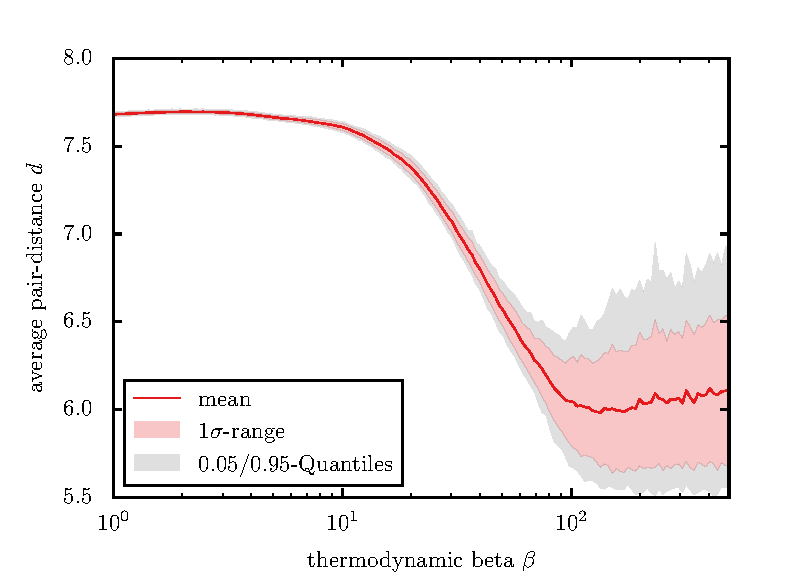
\includegraphics[width=\textwidth]{../report/figures/temp_dep_coulomb2d.pdf}
\end{frame}

\begin{frame}
	\frametitle{Results -- Coulomb 3D}
	\centering
	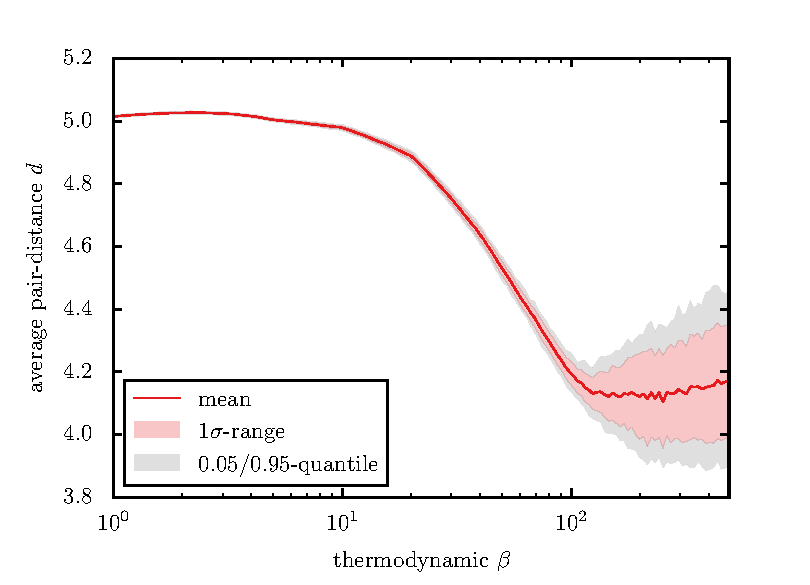
\includegraphics[width=\textwidth]{../report/figures/temp_dep_coulomb3d.pdf}
\end{frame}



% % % % % % % % % % % % Chris LJ 2D 3D & Visualizations

%Hier Folien
\begin{frame}{Results -- Lennard-Jones 2D}
	\pause
	\centering
	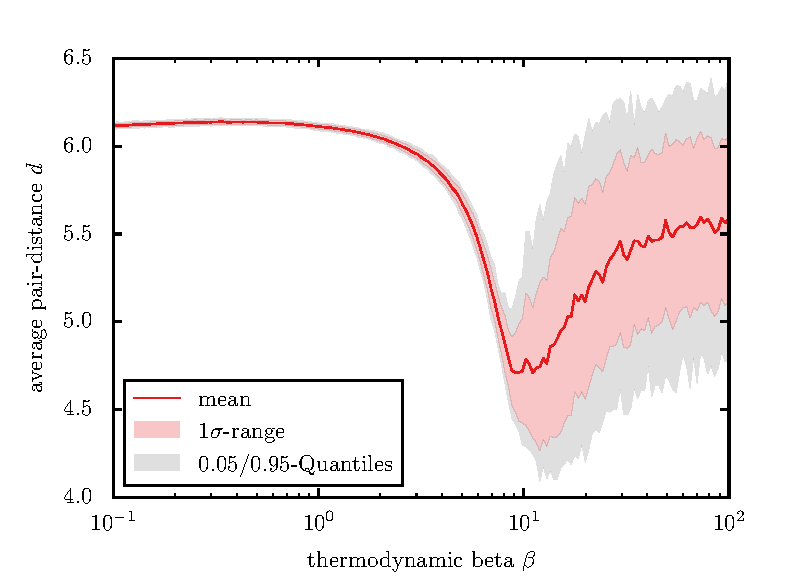
\includegraphics[width=\textwidth]{../report/figures/temp_dep_lennard_jones2d.pdf}
	\pause
	\put(-199.5,140){$\beta = 1$}
	\put(-186,152){\vector(0,1){17}}
\end{frame}

\begin{frame}
	\frametitle{Results -- Lennard-Jones 2D @ $\beta=1$}
	\centering
	\begin{columns}	
		\column[c]{0.6\textwidth}
		\begin{figure}
			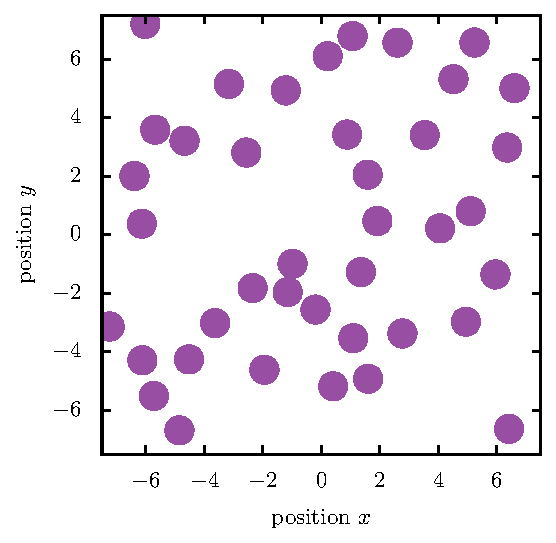
\includegraphics[width=\textwidth]{../report/figures/Beta_1_LJ.pdf}
		\end{figure}
		\column[c]{0.45\textwidth}
		\begin{itemize}
			\setlength{\itemsep}{1.5em}
			\item gaseous state
			\item like Coulomb case
			\item largest avg.\ pair-distance
		\end{itemize}
	\end{columns}
\end{frame}

\begin{frame}{Results -- Lennard-Jones 2D}
	\centering
	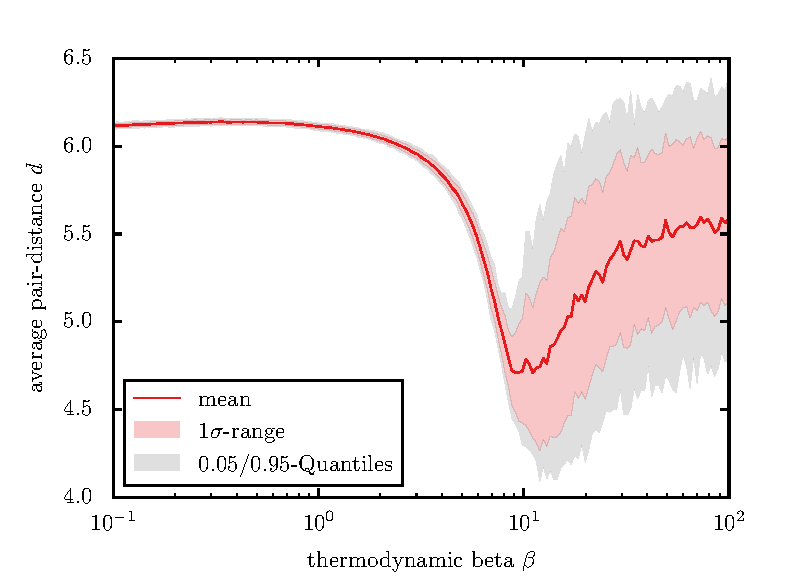
\includegraphics[width=\textwidth]{../report/figures/temp_dep_lennard_jones2d.pdf}
	\put(-146,180){$\beta = 5$}
	\put(-132,175){\vector(0,-1){17}}
\end{frame}

\begin{frame}
	\frametitle{Results -- Lennard-Jones 2D @ $\beta=5$}
	\centering
	\begin{columns}	
		\column[c]{0.6\textwidth}
		\begin{figure}
			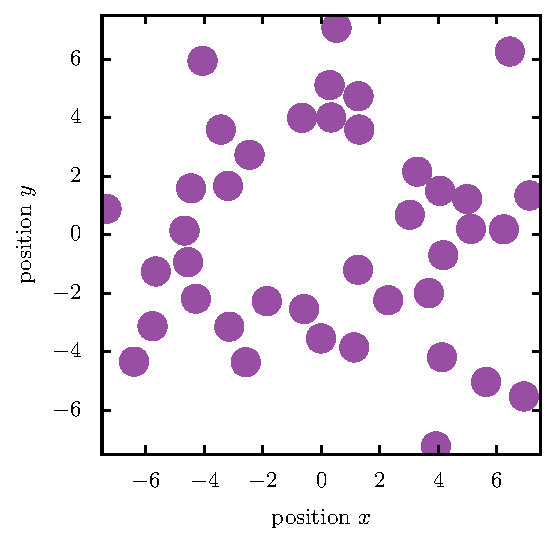
\includegraphics[width=\textwidth]{../report/figures/Beta_5_LJ.pdf}
		\end{figure}
		\column[c]{0.45\textwidth}
		\begin{itemize}
			\setlength{\itemsep}{1.5em}
			\item fluid-like state
			\item small clusters \& chains
		\end{itemize}
	\end{columns}
\end{frame}

\begin{frame}{Results -- Lennard-Jones 2D}
	\centering
	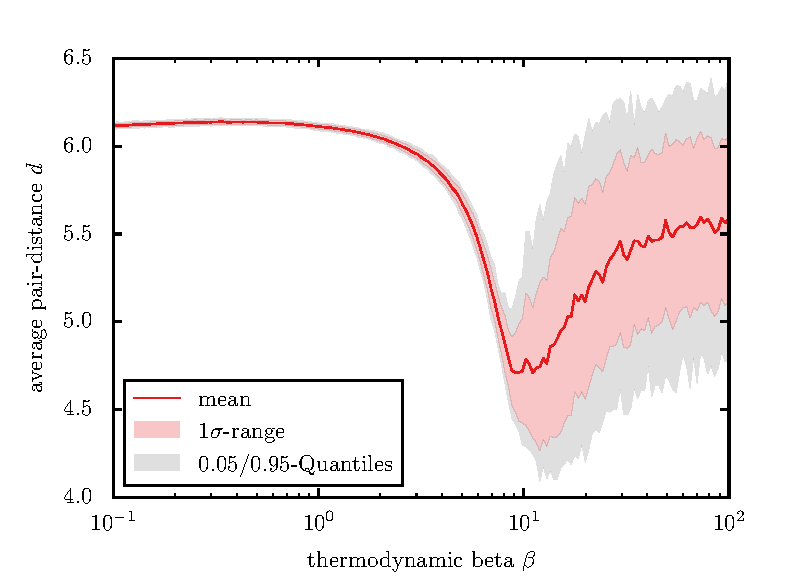
\includegraphics[width=\textwidth]{../report/figures/temp_dep_lennard_jones2d.pdf}
	\put(-124,50){$\beta = 10$}
	\put(-110,60){\vector(0,1){17}}
\end{frame}

\begin{frame}
	\frametitle{Results -- Lennard-Jones 2D @ $\beta=10$}
	\centering
	\begin{columns}	
		\column[c]{0.6\textwidth}
		\begin{figure}
			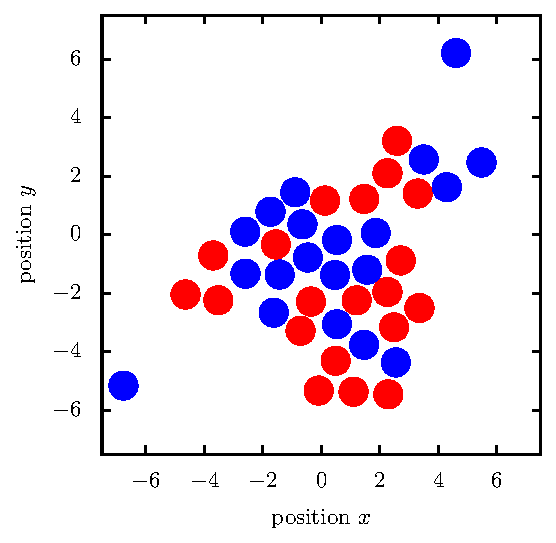
\includegraphics[width=\textwidth]{../report/figures/Beta_10_LJ.pdf}
		\end{figure}
		\column[c]{0.45\textwidth}
		\begin{itemize}
			\setlength{\itemsep}{1.5em}
			\item solid state
			\item single cluster
			\item smallest avg.\ pair-distance
			
		\end{itemize}
	\end{columns}
\end{frame}

\begin{frame}{Results -- Lennard-Jones 2D}
	\centering
	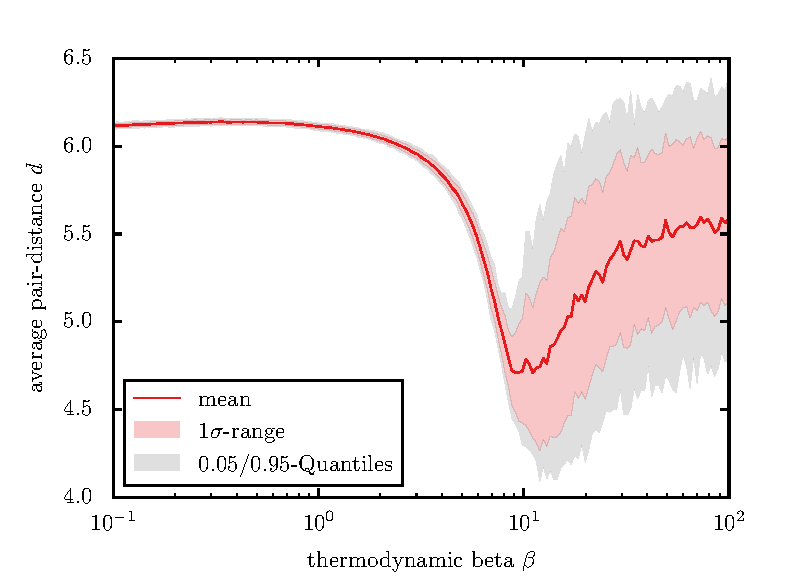
\includegraphics[width=\textwidth]{../report/figures/temp_dep_lennard_jones2d.pdf}
	\put(-75,165){$\beta = 100$}
	\put(-41,160){\vector(1,-2){10}}
\end{frame}

\begin{frame}
	\frametitle{Results -- Lennard-Jones 2D @ $\beta=100$}
	\centering
	\begin{columns}	
		\column[c]{0.6\textwidth}
		\begin{figure}
			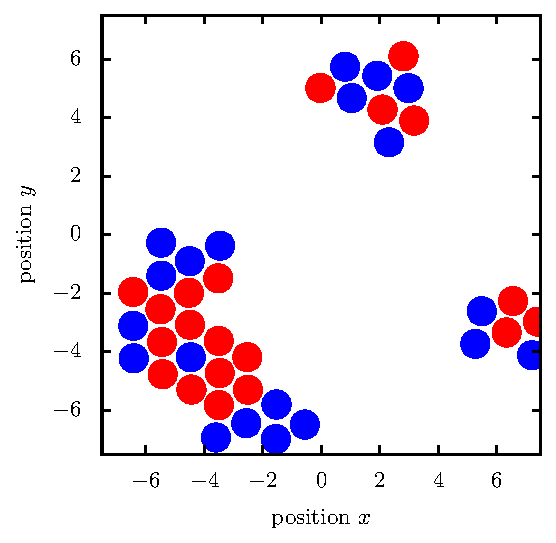
\includegraphics[width=\textwidth]{../report/figures/Beta_100_LJ.pdf}
		\end{figure}
		\column[c]{0.45\textwidth}
		\begin{itemize}
			\setlength{\itemsep}{1.5em}
			\item solid state
			\begin{itemize}
				\item triangular grid
			\end{itemize}
			\item multiple (independent) clusters
			\begin{itemize}
				\item increased avg.\ pair-distance
				\item source of large error
			\end{itemize}
		\end{itemize}
	\end{columns}
\end{frame}

\begin{frame}{Results -- Lennard-Jones 3D}
	\pause
	\centering
	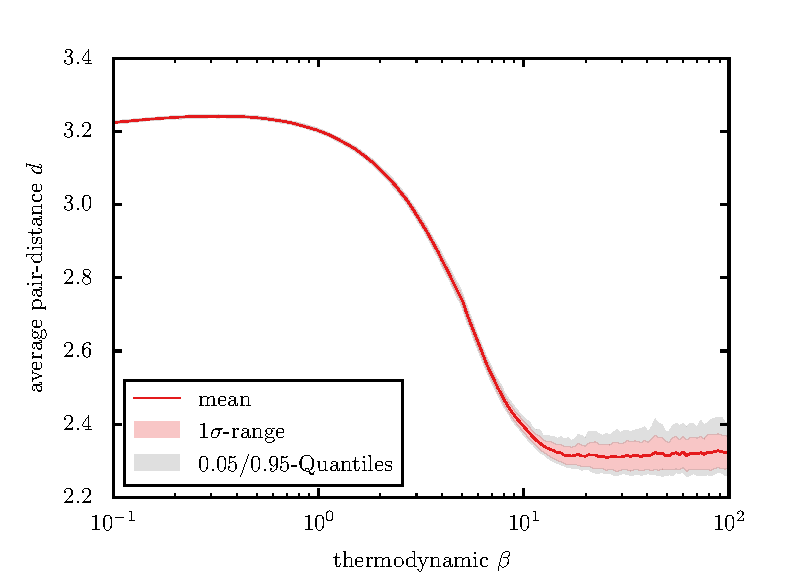
\includegraphics[width=\textwidth]{../report/figures/temp_dep_lennard_jones3d.pdf}
\end{frame}


% % % % % % % % % % % % Philip (+ Chris) Conclusion

%Hier Folien
\begin{frame}{Conclusion}
	\begin{itemize}
		\setlength{\itemsep}{1.5em}
		\item Metropolis algorithm -- good instrument to analyze ensembles
		\item easy implementation
		\item a lot of computation time $(d(\beta)$-plots)
		\item average pair-distance $\rightarrow$ phase transition
	\end{itemize}
\end{frame}

\begin{frame}{Thank you}
	\centering
	{\LARGE Thank you for your attention!}
\end{frame}

\end{document}